\documentclass{beamer}
\setbeamertemplate{navigation symbols}{}
\usepackage{beamerthemeshadow}


\begin{document}

\title{Active Learning}  
\author{Kacper Sokol}
\date{\today} 
\begin{frame}
\titlepage
\end{frame}




\begin{frame}
  \frametitle{Table of contents}
  \tableofcontents
\end{frame} 


\section{Concept of learning} 
  \subsection{Clustering}
  \begin{frame}
    \frametitle{Find two clusters} 
    \begin{figure}
      
\includegraphics[scale=.5]{graphics/presentation/clusters1} 
    \end{figure}
  \end{frame}

  \begin{frame}
    \frametitle{Find two clusters cont.} 
    \begin{figure}
      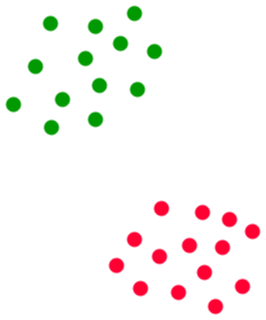
\includegraphics[scale=.5]{graphics/presentation/clusters1a} 
    \end{figure}
  \end{frame}

  \begin{frame}
    \frametitle{Find two clusters cont.} 
    \begin{figure}
      
\includegraphics[scale=.5]{graphics/presentation/clusters2} 
    \end{figure}
  \end{frame}

  \begin{frame}
    \frametitle{Find two clusters cont.} 
    \begin{figure}
      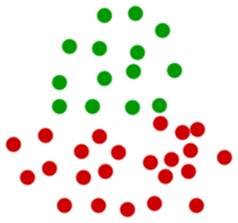
\includegraphics[scale=.5]{graphics/presentation/clusters2a} 
    \end{figure}
  \end{frame}

  \begin{frame}
    \frametitle{Find two clusters cont.} 
    \begin{figure}
      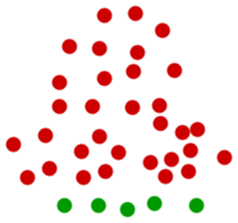
\includegraphics[scale=.5]{graphics/presentation/clusters2b} 
    \end{figure}
  \end{frame}

  \begin{frame}
    \frametitle{Find two clusters cont.} 
    \begin{figure}
      
\includegraphics[scale=.5]{graphics/presentation/clusters2c} 
    \end{figure}
  \end{frame}

  \begin{frame}
    \frametitle{Find two clusters cont.} 
    \begin{figure}
      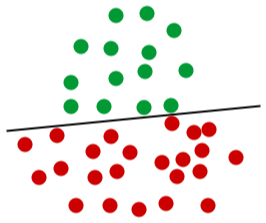
\includegraphics[scale=.5]{graphics/presentation/clusters2d} 
    \end{figure}
  \end{frame}

\subsection{The task}
  \begin{frame}
    \frametitle{Linear classifier}
    \begin{columns}
      \begin{column}{5cm}
        \begin{itemize}
          \item We are handling \textbf{binary classification}.
          \item The data are \textbf{linearly separable}.
          \item Therefore, our goal is to find two clouds of points separated by a straight line and make no error in separation.
        \end{itemize}
      \end{column}
      \begin{column}{5cm}
        \begin{figure}
          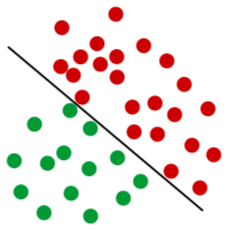
\includegraphics[scale=.4]{graphics/presentation/clusters2e} 
        \end{figure}
        \begin{itemize}
          \item green---a bike; red---a car
          \item x-axis---age of a person
          \item y-axis---distance form home to office/school
        \end{itemize}
      \end{column}
    \end{columns}
  \end{frame}

  \begin{frame}
    \frametitle{Linear classifier}
  \end{frame}

  \begin{frame}
    \frametitle{Supervised learning}
  \end{frame}

  \begin{frame}
    \frametitle{Active learning}
  \end{frame}


\section{Is it really exploration vs. exploitation?} 
\subsection{Multi-armed bandits as a workhorse}
  \begin{frame}
  \frametitle{MAB}
  \end{frame}

  \begin{frame}
  \frametitle{Ingredients of active learning}
  \end{frame}

  \begin{frame}
  \frametitle{numbered lists}
  \end{frame}

\begin{frame}\frametitle{numbered lists with pause}
\begin{enumerate}
\item Introduction to  \LaTeX \pause 
\item Course 2 \pause 
\item Termpapers and presentations with \LaTeX \pause 
\item Beamer class
\end{enumerate}
\end{frame}

\section{Section no.3} 
\subsection{Tables}
\begin{frame}\frametitle{Tables}
\begin{tabular}{|c|c|c|}
\hline
\textbf{Date} & \textbf{Instructor} & \textbf{Title} \\
\hline
WS 04/05 & Sascha Frank & First steps with  \LaTeX  \\
\hline
SS 05 & Sascha Frank & \LaTeX \ Course serial \\
\hline
\end{tabular}
\end{frame}


\begin{frame}\frametitle{Tables with pause}
\begin{tabular}{c c c}
A & B & C \\ 
\pause 
1 & 2 & 3 \\  
\pause 
A & B & C \\ 
\end{tabular} 
\end{frame}


\section{Section no. 4}
\subsection{blocs}
\begin{frame}\frametitle{blocs}

\begin{block}{title of the bloc}
bloc text
\end{block}

\begin{exampleblock}{title of the bloc}
bloc text
\end{exampleblock}


\begin{alertblock}{title of the bloc}
bloc text
\end{alertblock}
\end{frame}

\section{Section no. 5}
\subsection{split screen}

\begin{frame}\frametitle{splitting screen}
\begin{columns}
\begin{column}{5cm}
\begin{itemize}
\item Beamer 
\item Beamer Class 
\item Beamer Class Latex 
\end{itemize}
\end{column}
\begin{column}{5cm}
\begin{tabular}{|c|c|}
\hline
\textbf{Instructor} & \textbf{Title} \\
\hline
Sascha Frank &  \LaTeX \ Course 1 \\
\hline
Sascha Frank &  Course serial  \\
\hline
\end{tabular}
\end{column}
\end{columns}
\end{frame}

\subsection{Pictures} 
\begin{frame}\frametitle{pictures in latex beamer class}
% \begin{figure}
% \includegraphics[scale=0.5]{PIC1} 
% \caption{show an example picture}
% \end{figure}
\end{frame}

\subsection{joining picture and lists} 

\begin{frame}
\frametitle{pictures and lists in beamer class}
\begin{columns}
\begin{column}{5cm}
\begin{itemize}
\item<1-> subject 1
\item<3-> subject 2
\item<5-> subject 3
\end{itemize}
\vspace{3cm} 
\end{column}
\begin{column}{5cm}
\begin{overprint}
% \includegraphics<2>{PIC1}
% \includegraphics<4>{PIC2}
% \includegraphics<6>{PIC3}
\end{overprint}
\end{column}
\end{columns}
\end{frame}


\subsection{pictures which need more space} 
\begin{frame}[plain]
\frametitle{plain, or a way to get more space}
% \begin{figure}
% \includegraphics[scale=0.5]{PIC1} 
% \caption{show an example picture}
% \end{figure}
\end{frame}



\end{document}